\chapter{Einleitung}

\section{\acl{ARRI}}
Die Bachelorarbeit fand bei der Firma \ac{ARRI} statt. Gegründet wurde die Firma 1917 und auch nach über 100 Jahren Firmengeschichte liegt der Hauptsitz von \ac{ARRI} noch immer in München. 
Weltweit sind mittlerweile um die 1500 Mitarbeiter angestellt und die Firma ist einer der führenden Hersteller und Lieferanten in der Film- und Fernsehindustrie.

Die \ac{ARRI} Gruppe teilt sich in die folgenden fünf Geschäftsbereiche ein: Kamerasysteme, Licht, Postproduktion, Verleihservice und Operationskamerasysteme für die Medizin. \cite{arricorpinfo}

Das Thema dieser Bachelorarbeit wurde im Bereich Kamerasysteme in der Forschungs- und Entwicklungsabteilung erarbeitet.

\section{Kontext}
Um einen Überblick über das Umfeld der Arbeit zu bekommen, werden zunächst ein paar Grundlagen und auch die Funktionsweise einer Kamera betrachtet.


\subsection{Arbeitsumgebung}
Als Erstes soll auf die Zielplattform eingegangen werden. Die Wahl der Kamera ist auf eine \ac{ARRI} AMIRA gefallen, da deren Entwicklungsumgebung durch eine vorherige Arbeit bekannt ist. Zusätzlich ist sie nicht die aktuellste Kamera der Firma und somit ohne Probleme verfügbar. Allerdings ist die Hard- und Softwarearchitektur identisch zu den aktuellen Kameras, weshalb die Ergebnisse problemlos übertragen werden können.
Die AMIRA ist eine vielseitige Kamera, die für eine Einmannbedienung ausgelegt und mit einem Audioboard ausgestattet ist. Aus diesem Grund wird sie bei Dokumentationsfilmen und der elektronischen Berichtserstattung gerne verwendet. Zum Beispiel wird die \ac{ARRI} AMIRA bei Sportveranstaltungen der National Football League (NFL) in Amerika eingesetzt.\cite{arrinewsamira} 

\begin{figure}[!hbtp]
	\centering
	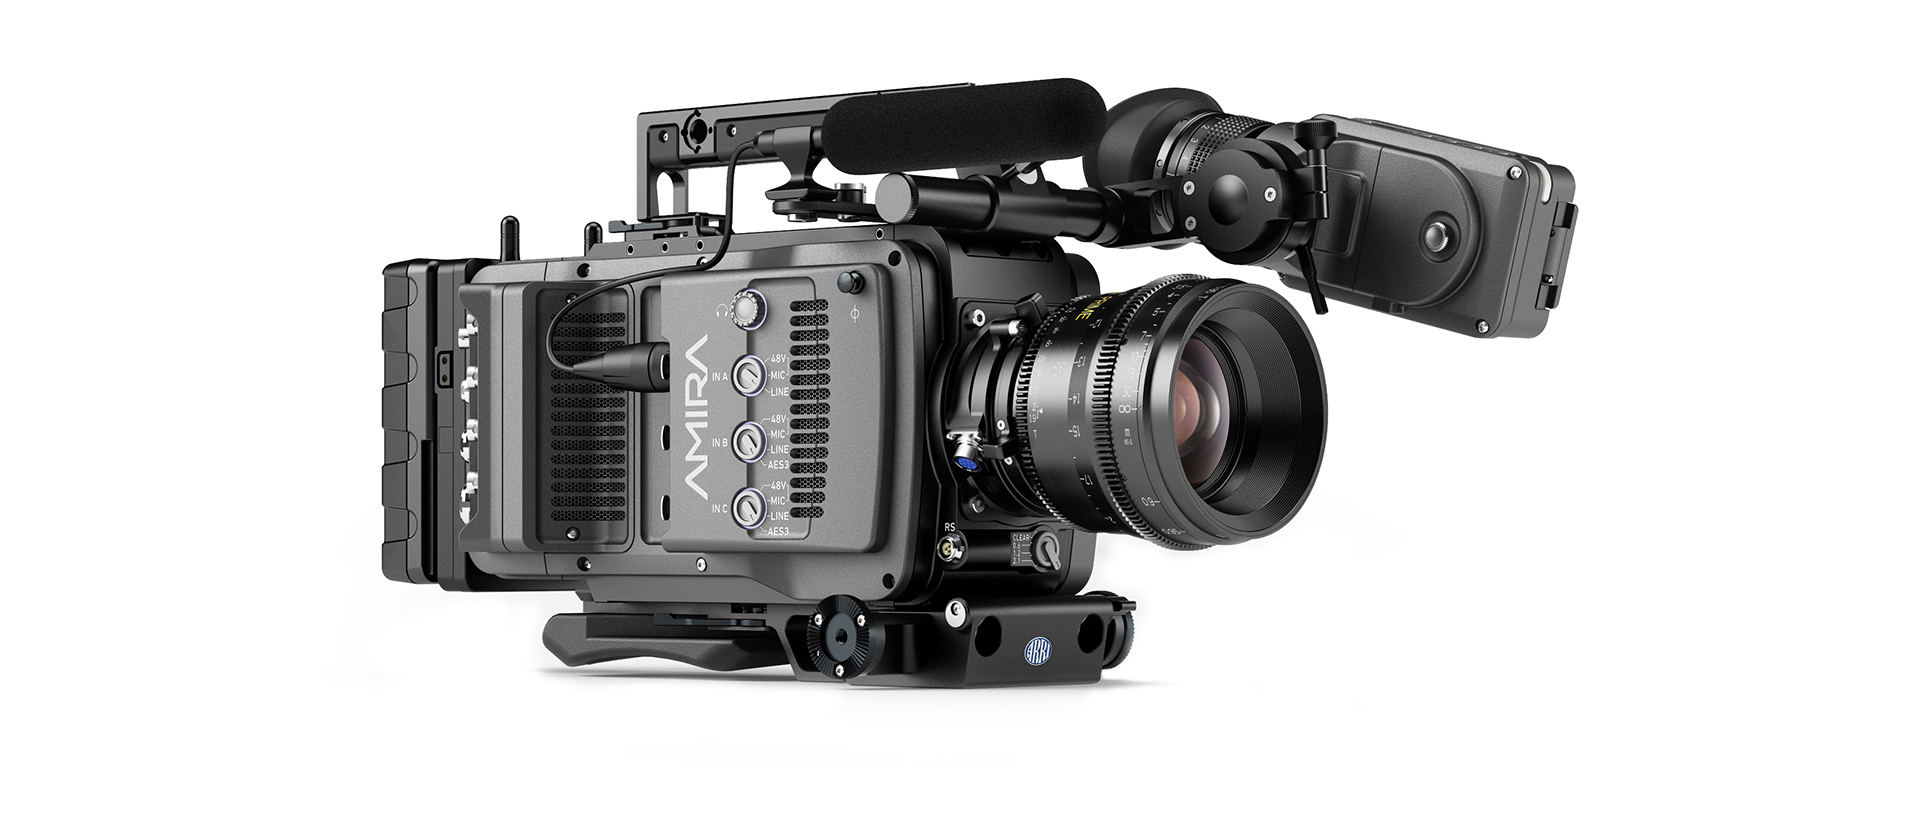
\includegraphics[width = 0.7\linewidth]{pictures/amira-product-image-data.jpg}
	\hspace*{0\textwidth}
	\caption{ARRI AMIRA}
	\caption*{siehe \cite{arriamira_bild}}
	\label{fig:amira}
\end{figure}  

Auch für Spielfilm- und Serienproduktionen wird  manchmal die \ac{ARRI} AMIRA eingesetzt, wodurch das breite Einsatzspektrum der Kamera noch deutlicher wird.
Als Beispiele sind hier der bayrische Eberhofer Krimi \glqq Sauerkrautkoma\grqq{} \cite{arrikrimi}, die Netflixserie \glqq The Ivory Game\grqq{} \cite{imdbivory} oder auch das Fernsehmagazin \glqq The Grand Tour\grqq{} \cite{imdbtour} zu nennen.
 
Die Kamera ist ein wichtiger Bestandteil in der Entwicklungsarbeit, da das regelmäßige Testen von Änderungen unerlässlich ist, um die Funktionalität beizubehalten und grobe Fehler rechtzeitig zu erkennen. Die aktuelle Software läuft über Linux auf der Kernelversion 5.3.7.

\subsection{Bildkette}\label{sec:bildkette}
In jeder Kamera wird das Eingangsbild von einem Sensor aufgenommen. Durch die Verarbeitungskette werden die Bilder vom Eingang bis zum Ausgang geleitet. In dieser Arbeit wird eine schematische Bildkette (siehe Abbildung~\ref{fig:bild}) zur Veranschaulichung weiter detailliert. Von der Quelle bis zur Senke läuft das Bild durch verschiedene Module, die für die Anpassung des Bilds sorgen. Die Ausgänge sind in diesem Fall die \ac{rec} und das \ac{sdi} zum Anzeigen des Videos.

\begin{figure}[!hbtp]
	\centering
	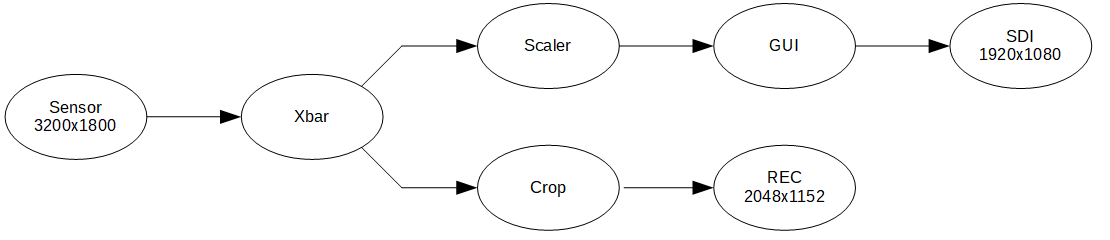
\includegraphics[width = \linewidth]{pictures/2019-11-17_Bildkette.png}
	\smallskip
	\caption{Schematische Bildkette}
	\label{fig:bild}
\end{figure} 

Direkt nach dem Sensor wird das Bild durch eine \ac{xbar} geleitet, hier wird das identische Bild in zwei Bildpfaden weitergeführt. Für die \acl{rec} wird das Bild im Crop zugeschnitten, damit wird nur ein bestimmter Bildausschnitt aufgezeichnet. In dem anderen Bildpfad wird, mithilfe des Scalers, das Bild kleiner skaliert. Nachdem eine \ac{gui} hinzugefügt worden ist, wird das Bild am \ac{sdi} Monitor ausgegeben. Hier ist, durch die Skalierung, das komplette Sensorbild einschließlich der eingefügten \ac{gui} zu sehen.

In dieser Arbeit wird nur das \ac{fpga}-Modul \ac{xbar} softwareseitig implementiert, da weitere Module sonst den Umfang der Arbeit überschreiten.

\subsection{Implementierung}
Bevor auf das erarbeitete Konzept eingegangen wird, soll kurz auf die Funktionsweise der Kamera und die aktuelle Implementierung eingegangen werden.

Die bildverarbeitende Hauptfunktionalität liegt im \ac{fpga}. Hier sind die Module entsprechend der Bildkette angeordnet und verbunden. Durch die Software werden bei den \ac{fpga} Modulen entsprechende Einstellungen vorgenommen.

Damit die Einstellungen auch zu dem Sensorbild passen, werden alle Module des \ac{fpga}s softwareseitig in dem \ac{geo} abgebildet. Das objektorientierte \gls{framework} führt hauptsächlich Berechnungen der Bildgrößen und Offsets durch. Nach der Änderung einer Größe in der Quelle oder Senke werden alle Module in der abgebildeten \gls{framework}bildkette aktualisiert und entsprechend der voreingestellten Parameter werden die Größen neu berechnet. Am Ende des Updates werden verschiedene Funktionen aufgerufen, welche die Register im \ac{fpga} entsprechend der Einstellungen setzen (siehe Abbildung~\ref{fig:newvsold} links).


\subsection{Problematiken}\label{sec:prob}
In der aktuellen Implementierung gibt es verschiedene Verbesserungsmöglichkeiten, die durch ein neues \gls{framework} gelöst werden sollen.

\paragraph*{Problem 1: Locking} Bei dem Zugriff auf ein Modul muss immer der \ac{fpga} gesperrt werden. Dadurch kann es passieren, dass es ein oder zwei \glspl{frame} dauert, bis alle Einstellungen in der Bildkette aktuell sind. Bei einem Livebild der Kamera ist dies besonders störend, da man die aktuelle Änderung erst später sieht. Da man beim Aufnehmen keine Änderungen am Sensorbild vornehmen kann fällt das Problem hier nicht ins Gewicht.

\paragraph*{Problem 2: Adressierung} Die Adressen für die \ac{fpga} Module müssen händisch eingetragen werden. Dadurch ist nicht nachvollziehbar, welcher Prozess in der Hardware Änderungen durchführt und somit die Fehlersuche extrem kompliziert und aufwendig. Zusätzlich steigt die Fehleranfälligkeit weiter an, da es passieren kann, dass die Software Einstellungen an eine Adresse schreibt, hinter der kein Modul liegt. In schlechtesten Fall werden die Register eines anderen Moduls beschrieben und es kommt zum Fehler in der Bildkette. 

\paragraph*{Problem 3: Kapslung} Die Größe der Registerbereiche der Module wird in der aktuellen Implementierung nicht weiter berücksichtigt. So kann es passieren, dass über den Bereich eines Moduls hinaus geschrieben wird. Auch dann kommt es zum Fehlerfall in der Bildkette, da andere Einstellungen überschrieben werden und so verloren gehen. \\



Im normalen Betrieb der Kamera können diese Fehlerfälle auftreten und somit in Filmproduktionen für Ausfällen sorgen. Dies ist mit der wichtigste Grund um die Software entsprechend anzupassen, sodass die Problematiken verschwinden.


\section{Konzept}\label{sec:konzept}
Durch das \ac{geo} wurde bereits ein großer Teil der Software umstrukturiert. Der letzte Schritt in der kompletten Umstrukturierung soll durch ein neues \gls{framework} gemacht werden. 
Die Probleme in der aktuellen Implementierung (siehe Kapitel~\ref{sec:prob}) 
durch das \gls{framework} behoben werden, zusätzlich sollen die Zugriffe der Software auf den \ac{fpga} übersichtlicher und wartbarer gestaltet werden.

\begin{figure}[!hbtp]
	\centering
	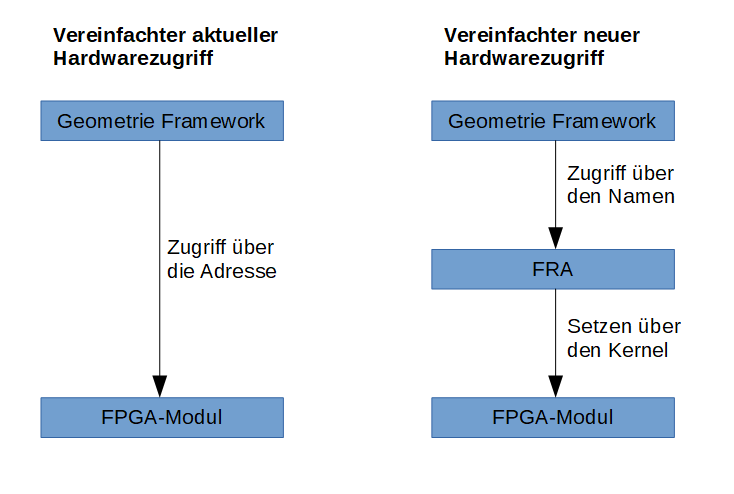
\includegraphics[width = 0.9\linewidth]{pictures/2019-11-17_ImplementierungNewvsOld.png}
	\smallskip
	\caption{Vereinfachte Darstellung des Zugriffs auf den \ac{fpga} in der aktuellen und der neuen Implementierung}
	\label{fig:newvsold}
\end{figure} 



Aktuell benötigen die Zugriffe auf den \ac{fpga} jedes Mal die Adressen der Module. Durch eine weitere Abstraktionsebene soll eine modulare Ansteuerung möglich werden und so die direkten Hardwarezugriffe über die Adressen aus dem Hauptcode eliminiert werden. Dadurch ist es möglich, jedes Modul individuell zu sperren und das Problem 1 (Locking) aus Kapitel~\ref{sec:prob} behoben.


In der neuen Abstraktionsebene, dem \ac{fra}, werden die Module im Kernel als Gerät angelegt und über \glspl{dateideskriptor} greift die Software auf den \ac{fpga} zu. Die Geräte werden mit der Adresse, der Größe, dem Namen und Typ des dahinterliegenden Modul beim Laden des \ac{fpga}s angelegt. Dieser Teil soll später generisch generiert werden und somit das zweite Problem (siehe Kapitel~\ref{sec:prob}) gelöst werden. Aber aufgrund von Abhängigkeiten zu anderen Entwicklungsteams wird es in dieser Arbeit nicht näher betrachtet.



Über die Modulnamen im vorhandenen \ac{geo} werden die \glspl{dateideskriptor} in der Software geöffnet und in einem \gls{handle} gespeichert. Damit wird im Hauptteil des Codes ein Zugriff ohne Adresse gewährleistet. Jeder laufende Prozess muss seinen eigenen \gls{dateideskriptor} öffnen und verwaltet somit sein eigenes \gls{handle}. Pro Modul kann lediglich eine begrenzte Anzahl von Deskriptoren geöffnet werden, geregelt wird dies durch den Kernel. 
Bei jedem Schreib- oder Lesezugriff auf ein Register wird überprüft, ob dieser innerhalb der angegebenen Modulgröße liegt. Damit ist es nicht mehr möglich über die Modulgrenzen hinweg zuschreiben und somit falsche Module zu beschreiben (Kapitel~\ref{sec:prob}: Problem 3).



Durch die neue Abstraktionsebene soll die Wartbarkeit sowie die Erweiterung der Kamerasoftware in Zukunft ohne tiefere Kenntnisse vom \ac{fpga} durch unterschiedliche Entwickler möglich werden. In der Abbildung~\ref{fig:newvsold} wird der Unterschied zwischen den Hardwarezugriffen zur Veranschaulichung der Funktionsweise vereinfacht dargestellt.



%\section{Hinführung zum Thema}\label{sec:thema}
%Damit die Kamera einwandfrei funktioniert müssen Firmware und Software zusammenspielen. Im \ac{geo} werden die verschiedenen Module aus dem \ac{fpga} abgebildet und entsprechend der Kameraeinstellungen die Bildgrößen berechnet. 

%In der Software werden dann in verschiedenen Funktionen die einzelnen Register im \ac{fpga} entsprechend gesetzt. Durch die aktuelle Implementierung können keine Module gleichzeitig im \ac{fpga} geupdatet werden. 


%Damit eine modulare Ansteuerung möglich wird, soll eine weitere Abstraktionsebene erstellt werden. Dieses sogenannte \ac{fra} soll die einzelnen Module im Kernel darstellen und entsprechend aus dem Userspace über \ac{ioctl} angesprochen werden können. Zusätzlich werden dann die direkten Hardwarezugriffe aus dem Hauptcode eliminiert. 

%Durch die neue Abstraktionsebene soll die Wartbarkeit sowie die Erweiterung der Kamerasoftware in Zukunft ohne tiefere Kenntnisse von \ac{fpga} durch unterschiedliche Entwickler möglich werden. 


%todo  und der zitate, erklärung das unterschiedliche nummern, da grundlegend identisch, neuere versionen allerdings mit mehr und ausfühlicheren kommentaren
